\section{Theory/Literature Review}\label{sec:2-theory}

Many of the individual things listed in this section are, in the land of computational/theoretical physics, very well established, meaning that no individual results are necessarily worthy of their own reference. Rather, see Ref.~\cite{Press_2007}, for instance, for descriptions of the computational techniques used and Ref.~\cite{peskin-schroeder} for descriptions of the physics theory.

\subsection{The Hard Scattering Process}

\subsubsection{Monte Carlo-Based Event Generators}

The driving force behind these types of simulation programs is the Monte Carlo algorithm, whose main purpose is to solve multi-dimensional integrals by averaging the integrand via randomly sampling points in the domain. Mathematically, what we are achieving is, given some integral

\begin{equation}
  I = \int_{t_1}^{t_2} \dd t \; f(t),
\end{equation}

we can approximate the result by

\begin{equation}
  I \approx \Delta t \Braket{f(t)} = \frac{\Delta t}{N} \sum_{\tau=1}^{\infty} f(\tau_i),
\end{equation}

where the $\tau_i$ lie in the range $(t_1,t_2)$. At this stage, we simply \textit{generate} $\tau_i$'s randomly, and the approximation will converge to the result after a sufficient number of evaluations. It's worth pointing out that we can randomly generate a number in the range $(0,1)$, then scale it to the domain, something like

\begin{equation}
  \tau_i = (t_2 - t_1)\rho_i + t_1,
\end{equation}

where $\rho_i$ is the random number, since the random number interface in most programming languages spit out a number between 0 and 1.

Of course, there are myriad other ways to solve integrals, but in particle physics, our problems and integrals are often formulated such that the dimensionality of the domain is large enough to dissuade the usage of quadrature-based integration schemes. Such integration schemes are more efficient in lower dimensions as they converge faster, but get much slower compared to Monte Carlo integration, whose rate of convergence increases in ``constant time'' in relation to the dimension. Of course, as an additional note, the reason this is a requirement at all is that the integrals we are faced with are very often mathematically impossible to solve analytically; e.g. the answer cannot be expressed in closed form.

Considering the physical process of the proton-proton collision, the starting point is the hard scattering process, which occurs immediately after the collision. The quantity we wish to calculate is the \textit{cross section} $\sigma$ for a particular relation which is, more or less, the probability for that reaction to occur. This is a quantity of interest to calculate because it can be measured and determined in the detectors, giving us a way to compare our theory with what is observed in real life.

To do this calculation, there are a few assumptions one must make. To understand this, we first know that protons are made up of quarks; one can think of the proton as a little ball with several quarks bouncing around inside. In the super high-energy collisions at the LHC, the assumption we make is that the proton's structure, i.e. \textit{where} the quarks are and their \textit{longitudinal} momenta (the portion of momenta of the quark that is in the direction of the proton's momenta) can be completely separated from the interactions between the individual proton's quarks. The point of doing this is that we are essentially ignoring the proton itself and only focusing on the interactions between the individual quarks. The location and momenta information is stored in what are called \textbf{parton distribution functions} (PDFs), and the information relative to the quark-quark interactions is stored in the \textit{partonic} cross section $\hat{\sigma}$, denoted with a hat instead to differentiate it from the total cross section.

To put this more formally, the total cross section is related to the sum of all possible interactions via the various quarks within the proton, proportional to the fraction of momentum they have compared to their host proton. Mathematically this looks like:

\begin{equation}
  \sigma(p(P_1) + p(P_2) \rightarrow X) = \int_0^1 \dd x_1 \int_0^1 \dd x_2 \; \sum_{i,j} f_{f_i}(x_1, \mu^2) f_{f_j}(x_2, \mu^2) \cdot \hat{\sigma}(f_i(x_1 P_1) + f_j(x_2 P_2) \rightarrow X).\label{eq:cross-section}
\end{equation}

This is a little dense, but here are what all the symbols mean: The left side is the cross section, representing two protons, one with momentum $P_1$ and the other with momentum $P_2$ colliding and leaving a generic final state $X$. On the right are the functions $f_i$ and $f_j$, which are the PDFs for quark $i$ and quark $j$. These are multiplied by the partonic cross section with quark $f_i$ (containing total momentum $x_1 P_1$, i.e. the fraction $x_1$ of the total momentum of its host proton $P_1$) interacting with quark $f_j$ and producing the aforementioned final state $X$. $\mu^2$ is energy scale of the process, since different quarks have different momentum fractions at different energy scales. Finally, these are convoluted together to get the final result.

The (differential) partonic cross section itself is given by:

\begin{equation}
  \dd\hat{\sigma}(f_i(x_1 P_1) + f_j(x_2 P_2) \rightarrow X) = \frac{1}{2\hat{s}} \abs{\mathcal{M}_{f_if_j \rightarrow X}}^2 \left( \prod_{k=1}^{N} \frac{\dd^3 p_k}{(2\pi)^3 2E_k} \right) (2\pi)^4 \delta^{(4)}(p_1 + p_2 + \sum_{k=1}^{N} p_k).
\end{equation}

Here, $E_i$ and $p_i$ are the energy and momentum of the $i$th parton, and the sum/products are over the $N$ different particles that may possibly be in the final state $X$. For this project, we are only considering $2\rightarrow2$ processes, in which two quarks interact and only two particles are produced in the final state. The calligraphic $\mathcal{M}$ is the \textit{amplitude}, and is specific to the process under consideration. Later, upon introducing the process we are modeling, the exact form of this amplitude will be shown. Everything apart from the amplitude in the expression is called the \textbf{phase space}, and essentially covers all energy/momentum configurations and inputs/outputs. In relation to the Monte Carlo algorithm, it is these phase space points that we randomly generate in the evaluation of this integral.


\subsubsection{The ``Hit-or-Miss'' Method}\label{sec:2-hit-or-miss}

In the event generation, when we are generating random phase space points and calculating our quantities of interest, we want to make sure that the events we are generating are in accordance with what would happen in the real world. In particular, if a phase space point gives a cross section significantly lower than others, it shouldn't necessarily be considered on the same footing as other events which are in principle far more likely to actually occur. One solution is to drag around every event's cross section so that we can take it into account later on. However, this extra baggage and additional computation can be inefficient.

One highly popular solution is dubbed the ``Hit-or-Miss'' method. This method involves finding the maximum ``weight'', which is the value of the integrand, during the calculation of the cross section; we shall call it $W_{\mathrm{max}}$. Then, when generating phase space points for the actual events, we only \textit{accept} an event (it ``hits'') with a probability of $w/W_{\mathrm{max}}$, where $w$ is the weight of that event (otherwise it ``misses''). One caveat to this method is that it doesn't work well if the function is not flat. One way to imagine this is to consider a simple function/curve on the 2D plane and generate random $x$-values. Hits are those that land in/below the curve, and misses land outside/above it. Clearly, if the function isn't very flat, this method doesn't work well.

Sometimes, we are able to circumvent this by applying a transformation/change of variables. One particularly good example is the Breit-Wigner peak, modeled by the function

\begin{equation}
  F(m^2) = \frac{1}{(m^2 - M^2)^2 + M^2\Gamma^2}.
\end{equation}

This function is used to model resonances, which are essentially unstable particles, where $m^2$ is the center of mass energy that produces the resonance, $M$ is the actual mass of the resonance, and $\Gamma$ is the decay width of the resonance, which is inversely proportional to the lifetime of the particle. We are often interested in integrals of this function:

\begin{equation}
  I = \int_{M_{\mathrm{min}}^2}^{M_{\mathrm{max}}^2} \dd m^2 \; \frac{1}{(m^2 - M^2)^2 + M^2\Gamma^2}.
\end{equation}


\begin{figure}[ht]
  \centering
  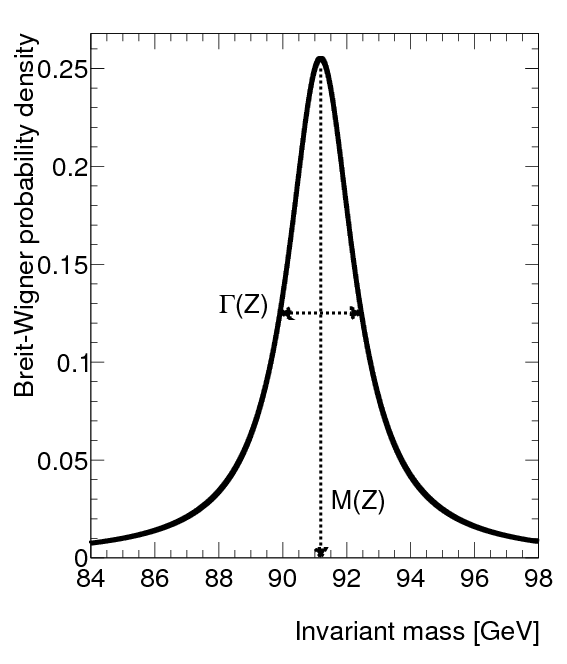
\includegraphics[width=0.4\linewidth]{./res/gfx/breit-wigner.png}
  \caption{Example of the Breit-Wigner distribution.}
  \label{fig:BreitWigner}
\end{figure}


An example plot is given in Fig.~\ref{fig:BreitWigner}; the peak is at $\qty{91}{\GeV}$, which is the mass of the $Z$-boson, and the width $\Gamma$ is, again, related to its lifetime. Obviously, such a function would be a particularly bad candidate for the hit-or-miss method. However, if we made the change of variables to $\rho$ like so:

\begin{equation}
  m^2 = M\Gamma\tan\rho + M^2,
\end{equation}

our integral turns into

\begin{equation}
  I = \frac{1}{M\Gamma} \int_{\rho_{\mathrm{min}}}^{\rho_{\mathrm{max}}} \dd\rho,
\end{equation}

which is perfectly flat, thus removing any variance and making it a perfect candidate for the hit-or-miss method. Unfortunately, we are probably never going to be able to find a transformation that is perfect like this one, but we can often get very close, which is more than good enough, especially considering that we are already truncating things at leading-order anyways.

At this point, once we have a set of phase space points that passed the hit-or-miss selection, we can generate events by simply generating some momenta in accordance with the phase space information. These will correspond to particles that, in a real simulation, would be produced immediately after the collision.


\subsection{Parton Showering/Hadronization Process}

The calculation of hard scattering cross section and generation of events in accordance with the cross sections is a bit more simple than the parton showering process, since the former involves a very general Monte Carlo algorithm. Parton showering is more directly based within the physics itself. As such, the results presented in this section are a conglomeration of results taken from the \textsc{Pythia8} and \textsc{Herwig7} manuals \cite{PYTHIA8DOC,HERWIGDOCS}, as well as from a condensed ``tutorial'' given in \cite{PYRESIAS}.

The main physics behind parton showering is the idea that, immediately after the main collision, quarks will fly out with super high energies. In general, quantum mechanics dictates that particles want to release their excess energy and drop down to their ``ground'' state. The highly energetic quarks are certainly not in their ground state, and one method by which they release this additional energy is by emitting gluons. In general, any given quark can do this several times, and the gluon may decay into a quark/anti-quark pair, which may emit gluons again, and so on. This leads to a ``shower'' or ``jet'' of particles in the final state.

We consider the simple case of a single quark emitting single gluons one at a time, because anything further becomes extremely complex. The main mathematical structure related to the emission of gluons/photons is the \textbf{Sudakov form factor}, defined like so:

\begin{equation}
  \Delta(t_0,t) \equiv \exp\left[ -\int_{t_0}^t \dd t' \; \Gamma(t') \right],
\end{equation}

where $t_0$ is the quark's initial energy, and $t$ is its final energy when it can no longer emit gluons. The function $\Gamma(t')$ is defined as:

\begin{equation}
  \Gamma(t') \equiv \frac{1}{t'} \int_{z_-}^{z_+} \dd z \; \frac{\alpha_s}{2\pi}P_{g \leftarrow q}(z),\label{eq:2-theory-gamma}
\end{equation}

where the $t'$ is simply to differentiate from the main integration variable. $\alpha_s$ is the strong coupling constant, characterizing how strongly quarks and gluons interact with each other, $z^-$ and $z^+$ are arbitrary limits on the max/min energy of the quark, and $P$ is called the \textbf{splitting function}, which essentially gives the probability for the quark to emit the gluon (it is similar-ish to PDFs, but a bit simpler). It is defined like so:

\begin{equation}
  P_{g \leftarrow q}(z) = C_F \frac{1 + z^2}{1 - z}\label{eq:2-theory-splittingfn}
\end{equation}

where $C_F=4/3$ is a group-theoretical constant\footnote{Physicists, for one reason or another, often like to leave things like this as general as possible. The value it takes is nearly always $4/3$.} and $z$ is the momentum fraction of the gluon (analogous to $x$ from the PDFs). The interpretation of the Sudakov form factor is that it gives the probability that the quark doesn't emit a gluon as we evolve from the initial scale $t$ to the cutoff scale $t_0$. By evolve, we simply mean as the quark loses energy via anything else that may happen in the reaction, such as collisions with other particles, for instance. It may seem like this is reversed: why are we calculating when it \textit{doesn't} emit a gluon?

Too see why we do this, we consider how this is implemented in a program. What we do is scale the Sudakov factor to the range $[0,1]$, calculate it for a given $t$ and $t_0$, then generate a random number also in the range $[0,1]$. The larger the value of the Sudakov factor, the less likely it is to emit a gluon. So, if our random, number lies \textit{above} the value of the Sudakov, we \textit{do} have an emission, otherwise we don't. We then solve for $t$ by inverting $\Delta(t,t_0)$ to calculate at what point this emission occurs, then continue on from there, where now the quark's energy has been reduced to whatever energy it emitted the gluon at. Further, we need to determine/consider the kinematics of the emitted gluon, specifically $z$, the fraction of the parton's momentum it carries. This is done by solving for $z$ by inverting $\Gamma(t)$.

There are a few issues with solving for $t$ and $z$, and that is the fact that both require evaluating inverses or integrals of functions which are, in general, very hard to integrate or invert. There is an algorithm to largely resolve this, called the \textit{Sudakov veto algorithm}, which resembles the hit-or-miss method discussed in the previous section. The main idea is that for the functions that we have to invert, we take away some of the complexity by defining new variables that are \textit{overestimates} of the original variable for the entire domain such that the function is more easily invertable. Of course, this implies a higher ``acceptance'' of events or of emissions -- the probabilities are then ``fixed'' by only accepting proposed events according a ratio of the original variable's value to the overestimate's value.

As an example, an overestimate of the splitting function would be given by

\begin{equation}
  \hat{P}(z) = C_F \frac{2}{1-z},\label{eq:2-theory-splittingfnover}
\end{equation}

since $z \in [0,1]$ so the numerator in Equation~\eqref{eq:2-theory-splittingfn} will never be larger than 2, meaning that Equation~\eqref{eq:2-theory-splittingfn} overestimates the splitting function everywhere. This overestimate is now much easier to invert and solve for $z$.

\subsubsection{The Cutoff \texorpdfstring{$t_0$}{t0}}\label{sec:2-theory-cutoff}

Lastly, we explain why we need some cutoff scale. We already mentioned beforehand that the quark emits gluons so that it returns to its ground state. This isn't \textit{wrong}, in general, but for quarks, it is a little different. In the introduction, it was mentioned that the force quarks experience is the reverse of the electromagnetic force: it becomes more strongly attracted to quarks at \textit{larger} distances. Energies, in general, in the quantum world, are directly related to distances (hence why we say we are probing the universe at high energies, as this is equivalent to saying we are probing the universe at the smallest distance scales). So, once the quark releases enough energy, the distance scales associated with the system are sufficent that the coupling between quarks grow enough to hardonize, e.g. form protons. There is a universally understood energy(/distance) scale at which this occurs, roughly $\qty{~1}{\GeV}$~\cite{Hoang_2024}.

At this point, then, our perturbation theory approach breaks down, as the series in Equation~\eqref{eq:1-intro-perturbation} no longer converges since $\lambda$, which is the coupling strength, is so high. Therefore, the entire theory on which this method is based breaks down,\footnote{The splitting functions(s) (Equation~\eqref{eq:2-theory-splittingfn}) are calculated via perturbation theory; they would be completely invalid.} and we cannot continue calculations below this limit without producing results that are inconsistent with the real world. Additionally, it is obvious that if we let $t$ get too small, the factor of $1/t$ in Equation~\eqref{eq:2-theory-gamma} will diverge, which we must avoid.

%%% Local Variables:
%%% mode: LaTeX
%%% TeX-master: "../../FinalMilestone"
%%% End:
